% Cultural Differences between the USA and Austria
% Compile with: latexmk -pdf cultural_differences.tex
\documentclass[aspectratio=169,11pt]{beamer}

\usepackage[T1]{fontenc}
\usepackage{lmodern}
\usepackage{booktabs}
\usepackage{tikz}
\usetikzlibrary{shapes.geometric,positioning,calc}
\usepackage{pgfplots}
\pgfplotsset{compat=1.18}
\usepackage[most]{tcolorbox}
\graphicspath{{images/}}

% ---------- Colors ----------
\definecolor{navy}{HTML}{1C2541}
\definecolor{oldred}{HTML}{B22234}
\definecolor{oldblue}{HTML}{3C3B6E}
\definecolor{ink}{HTML}{2B2B2B}
\definecolor{muted}{HTML}{8A8F98}
\definecolor{paper}{HTML}{FFFFFF}
\definecolor{austria}{HTML}{C8102E}

% ---------- Minimal theme ----------
\setbeamertemplate{navigation symbols}{}
\setbeamercolor{normal text}{fg=ink, bg=paper}
\setbeamercolor{structure}{fg=navy}
\setbeamercolor{frametitle}{fg=navy}
\setbeamercolor{alerted text}{fg=oldred}
\setbeamercolor{footnote}{fg=muted}
\setbeamerfont{frametitle}{size=\Large, series=\bfseries}
\setbeamertemplate{itemize item}{\color{oldred}\textbullet}
\setbeamertemplate{itemize subitem}{\color{muted}--}
\setbeamertemplate{enumerate item}{\color{oldred}\insertenumlabel.}
\setbeamersize{text margin left=1.1cm, text margin right=1.1cm}

\setbeamertemplate{frametitle}{%
  \vspace*{0.5cm}%
  \usebeamerfont{frametitle}\usebeamercolor[fg]{frametitle}\insertframetitle\par
  \vspace{0.15cm}{\color{navy!15}\rule{\textwidth}{0.4pt}}\par}

\setbeamertemplate{footline}{%
  \hfill{\tiny\color{muted}\insertframenumber}\hspace*{0.6cm}\vspace*{0.35cm}}

% Plain divider at the start of each section
\AtBeginSection{%
  \begin{frame}[plain,noframenumbering]
    \centering
    {\LARGE\bfseries\color{navy}\insertsection}\\[0.6em]
    {\color{oldred}\rule{1.5cm}{0.8pt}}
  \end{frame}}

% "Think" question slides
\newenvironment{thinkframe}{%
  \begin{frame}[plain,noframenumbering,environment=thinkframe]\centering\Large}{\end{frame}}

% ---------- Helpers ----------
% Small grey source line at the bottom of a frame
\newcommand{\source}[1]{%
  \begin{tikzpicture}[remember picture,overlay]
    \node[anchor=south west, font=\tiny, text=muted, text width=0.85\paperwidth, align=left]
      at ($(current page.south west)+(0.6cm,0.25cm)$) {#1};
  \end{tikzpicture}}

% Quote box with a thin red rule on the left
\newtcolorbox{textquote}[1][]{%
  enhanced, breakable=false, frame hidden, boxrule=0pt, sharp corners,
  colback=navy!4, borderline west={2pt}{0pt}{oldred},
  left=10pt, right=8pt, top=6pt, bottom=6pt, fontupper=\itshape, #1}

% US flag (hoist = #1)
\newcommand{\usflag}[1]{%
  \begin{tikzpicture}[x=#1, y=#1]
    \def\fly{1.9}
    \foreach \i in {0,...,12} {
      \pgfmathsetmacro{\c}{mod(\i,2)==0 ? 1 : 0}
      \ifdim\c pt=1pt
        \fill[oldred] (0,{1-(\i+1)/13}) rectangle (\fly,{1-\i/13});
      \else
        \fill[white] (0,{1-(\i+1)/13}) rectangle (\fly,{1-\i/13});
      \fi
    }
    \def\cw{0.76} \def\ch{0.5385}
    \fill[oldblue] (0,{1-\ch}) rectangle (\cw,1);
    \foreach \r in {1,...,9} {
      \pgfmathsetmacro{\isodd}{mod(\r,2)}
      \ifdim\isodd pt=1pt
        \foreach \k in {0,...,5}
          \node[star, star points=5, star point ratio=2.618, fill=white, inner sep=0pt,
                minimum size=0.0616*#1] at ({(2*\k+1)*\cw/12},{1-\r*\ch/10}) {};
      \else
        \foreach \k in {0,...,4}
          \node[star, star points=5, star point ratio=2.618, fill=white, inner sep=0pt,
                minimum size=0.0616*#1] at ({(2*\k+2)*\cw/12},{1-\r*\ch/10}) {};
      \fi
    }
    \draw[ink!30, line width=0.3pt] (0,0) rectangle (\fly,1);
  \end{tikzpicture}}

% Agree/disagree spectrum for the activity
\newcommand{\spectrum}{%
  
\begin{tikzpicture}
    \shade[left color=oldblue, right color=oldred, rounded corners=2pt] (0,0) rectangle (11,0.18);
    \node[anchor=north, font=\small, text=oldblue] at (0,-0.15) {Strongly disagree};
    \node[anchor=north, font=\small, text=muted] at (5.5,-0.15) {Neutral};
    \node[anchor=north, font=\small, text=oldred] at (11,-0.15) {Strongly agree};
    \fill[paper, draw=muted] (5.5,0.09) circle (2.5pt);
  \end{tikzpicture}}

\newcommand{\statement}[2]{%
  \begin{frame}[plain]
    \vfill
    \begin{center}
      {\small\color{muted}Statement #1 of 5}\\[1.2em]
      {\LARGE\bfseries #2}
    \end{center}
    \vfill
    \begin{center}\spectrum\end{center}
    \vspace{1.2cm}
  \end{frame}}

% ---------- Title ----------
\title{Cultural Differences}
\subtitle{The USA and Austria}
\author{}
\date{}

\begin{document}

\begin{frame}[plain]
  \begin{columns}[c]
    \begin{column}{0.55\textwidth}
      {\fontsize{30}{34}\selectfont\bfseries\color{navy} Cultural\\Differences}\\[0.8em]
      {\Large\color{muted} The USA and Austria}\\[0.6em]
      {\color{oldred}\rule{3cm}{1.5pt}}
    \end{column}
    \begin{column}{0.4\textwidth}
      \centering\usflag{2.9cm}
    \end{column}
  \end{columns}
\end{frame}

% =====================================================================
\section{Warm-up}

\begin{frame}{Warm-up}
  \centering
  {\LARGE What do you know about American culture?}
\end{frame}

% =====================================================================
\section{The Pledge of Allegiance}

\begin{frame}{The Pledge of Allegiance}
  \begin{columns}[c]
    \begin{column}{0.52\textwidth}
      \large\linespread{1.25}\selectfont
      I pledge allegiance to the Flag\\
      of the United States of America,\\
      and to the Republic\\
      for which it stands,\\
      one Nation under God,\\
      indivisible,\\
      with liberty and justice for all.

      \vspace{1em}
      \small\color{muted}\itshape Stand, face the flag, right hand over your heart.
    \end{column}
    \begin{column}{0.44\textwidth}
      \centering\usflag{3.1cm}
    \end{column}
  \end{columns}
\end{frame}

\begin{frame}{Reflection}
  \begin{itemize}\setlength{\itemsep}{1.2em}
    \item What did that feel like?
    \item Do you think this is still practiced in schools?
    \item What time period do you think this is from?
  \end{itemize}
\end{frame}

\begin{frame}{History behind the Pledge}
  \begin{itemize}\setlength{\itemsep}{0.6em}
    \item \textbf{1885:} First version by Captain George Thatcher Balch, a Union Army officer in the Civil War
      \begin{itemize}
        \item \emph{``We give our heads and our hearts to God and our country; one country, one language, one flag!''}
      \end{itemize}
    \item \textbf{1892:} Francis Bellamy, a Baptist minister, writes a new version for the 400th anniversary of Columbus's arrival in America
      \begin{itemize}
        \item Published in \emph{The Youth's Companion}, a children's magazine that also sold flags to schools
      \end{itemize}
    \item \textbf{1923--24:} ``my Flag'' becomes ``the Flag of the United States of America''
      \begin{itemize}
        \item So that immigrants would not be thinking of the flag of their home country
      \end{itemize}
  \end{itemize}
\end{frame}

\begin{frame}{History behind the Pledge}
  \begin{columns}[T]
    \begin{column}{0.56\textwidth}
      \begin{itemize}\setlength{\itemsep}{0.6em}
        \item \textbf{1942:} Congress officially adopts the Pledge
        \item The original ``Bellamy salute'' (right arm stretched out) looked too much like the Nazi salute
          \begin{itemize}
            \item Replaced with the \alert{hand over the heart}
          \end{itemize}
        \item \textbf{Flag Day, 1954:} President Eisenhower adds \alert{``under God''}
          \begin{itemize}
            \item Cold War: setting America apart from ``godless'' Soviet communism
          \end{itemize}
      \end{itemize}
    \end{column}
    \begin{column}{0.4\textwidth}
      \centering
      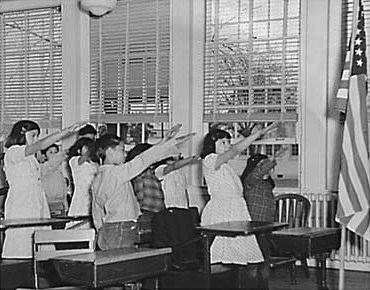
\includegraphics[width=\linewidth]{bellamy_salute.jpg}\\[0.2em]
      {\tiny\color{muted} Students giving the Bellamy salute, 1941}\\[0.6em]
    \end{column}
  \end{columns}
\end{frame}

\begin{frame}{The Pledge over time}
  \centering
  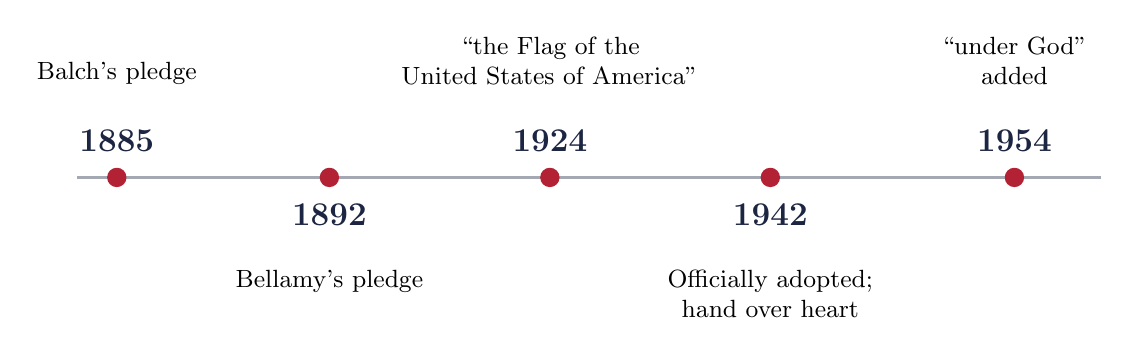
\begin{tikzpicture}[x=1cm, y=1cm]
    \draw[navy!40, line width=1.2pt] (0,0) -- (13,0);
    \foreach \x in {0.5, 3.2, 6.0, 8.8, 11.9}
      \fill[oldred] (\x,0) circle (3.5pt);
    \node[font=\bfseries\large, text=navy, above=6pt] at (0.5,0) {1885};
    \node[font=\small, align=center, above=30pt] at (0.5,0) {Balch's pledge};
    \node[font=\bfseries\large, text=navy, below=6pt] at (3.2,0) {1892};
    \node[font=\small, align=center, below=30pt] at (3.2,0) {Bellamy's pledge};
    \node[font=\bfseries\large, text=navy, above=6pt] at (6.0,0) {1924};
    \node[font=\small, align=center, above=30pt] at (6.0,0) {``the Flag of the\\United States of America''};
    \node[font=\bfseries\large, text=navy, below=6pt] at (8.8,0) {1942};
    \node[font=\small, align=center, below=30pt] at (8.8,0) {Officially adopted;\\hand over heart};
    \node[font=\bfseries\large, text=navy, above=6pt] at (11.9,0) {1954};
    \node[font=\small, align=center, above=30pt] at (11.9,0) {``under God''\\added};
  \end{tikzpicture}
\end{frame}

\begin{frame}{What does this show about American culture?}
  \begin{columns}[c]
    \begin{column}{0.5\textwidth}
      \begin{itemize}\setlength{\itemsep}{1em}
        \item Loyalty and patriotism
        \item Unity? --- ``one Nation \ldots\ indivisible''
        \item Religion in public life --- ``under God''
        \item Turning immigrants into Americans
      \end{itemize}
    \end{column}
    \begin{column}{0.46\textwidth}
      \centering
      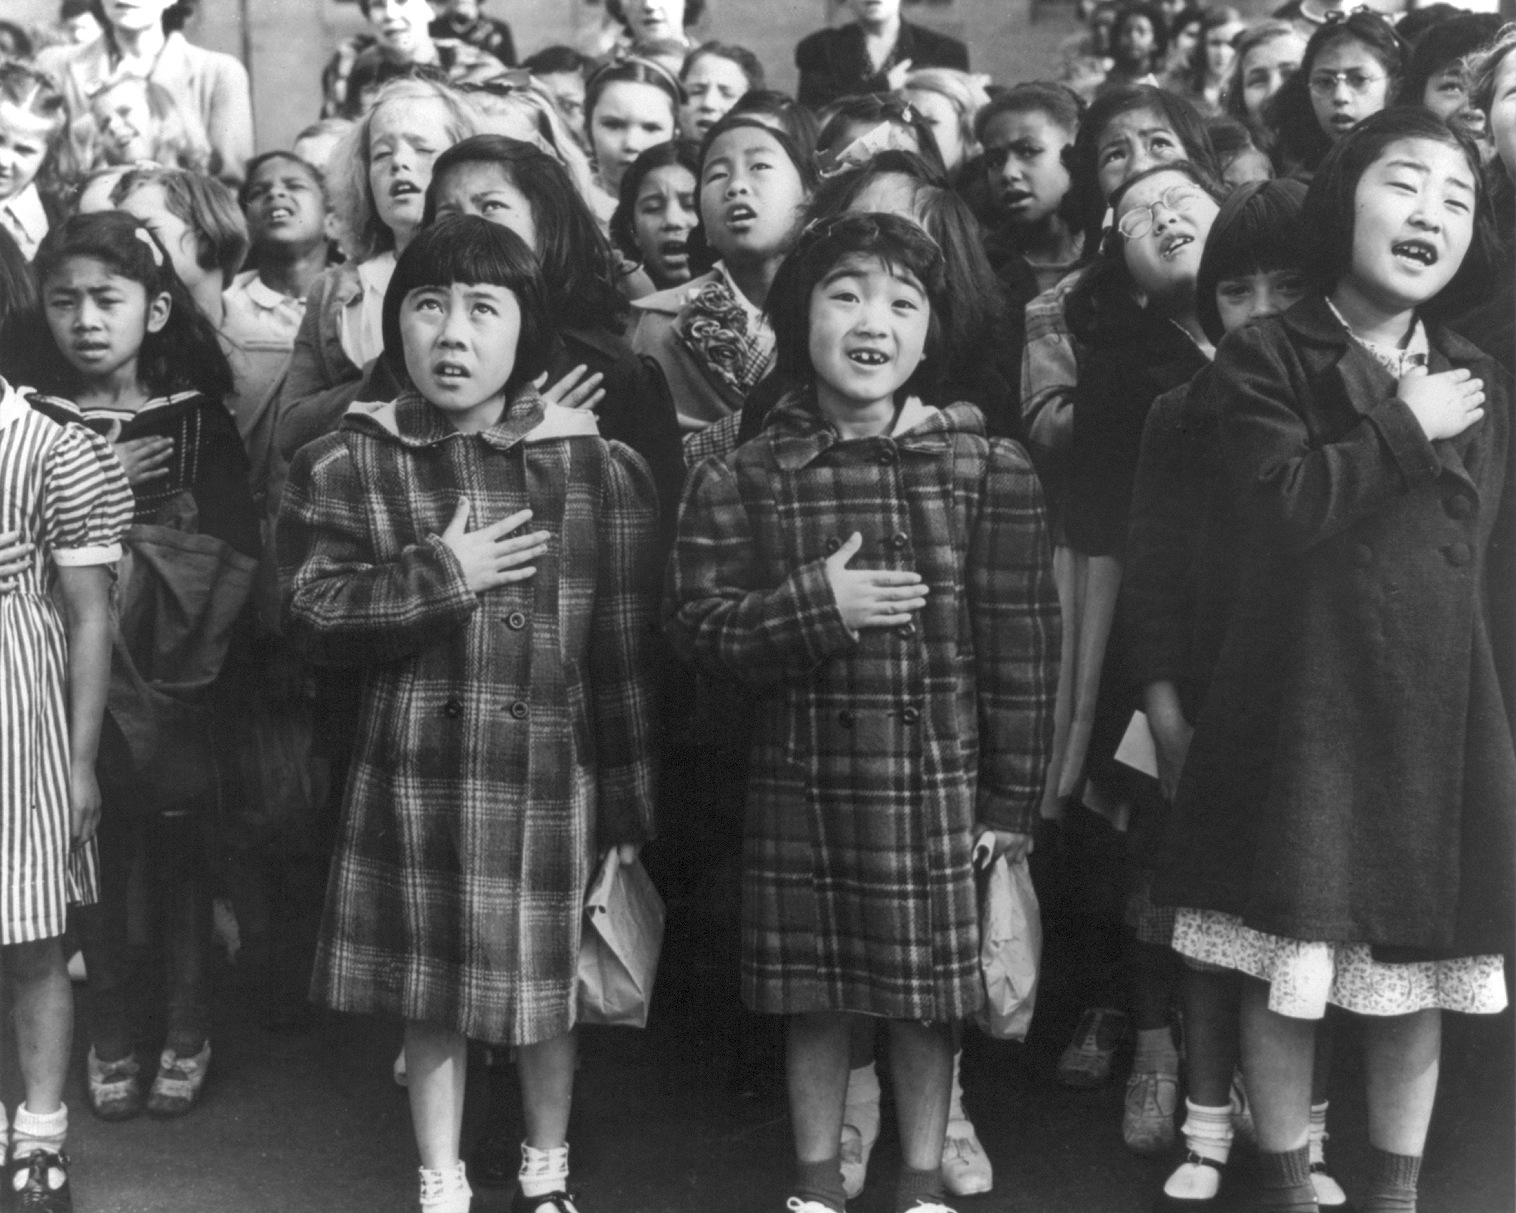
\includegraphics[width=\linewidth]{pledge_1942.jpg}\\[0.2em]
      {\tiny\color{muted} San Francisco, 1942. Weeks later, many of these Japanese American children were sent to internment camps. Photo: Dorothea Lange\par}
    \end{column}
  \end{columns}
\end{frame}

\begin{frame}{Legal challenges}
  \begin{columns}[T]
    \begin{column}{0.58\textwidth}
      \small
      \begin{itemize}\setlength{\itemsep}{0.4em}
        \item \textbf{1940:} \emph{Minersville v.\ Gobitis} --- schools \emph{may} force students to recite the Pledge; Jehovah's Witness children who refused were expelled
        \item \textbf{1943:} \emph{West Virginia State Board of Education v.\ Barnette} --- the Supreme Court reverses itself: reciting the Pledge \alert{cannot be compulsory}
        \item \textbf{2004:} \emph{Elk Grove v.\ Newdow} --- a father challenges ``under God''; the Court dismisses the case on a technicality
        \item \textbf{Today:} most states require schools to lead the Pledge daily --- but students may stay silent
      \end{itemize}
    \end{column}
    \begin{column}{0.38\textwidth}
      \centering
      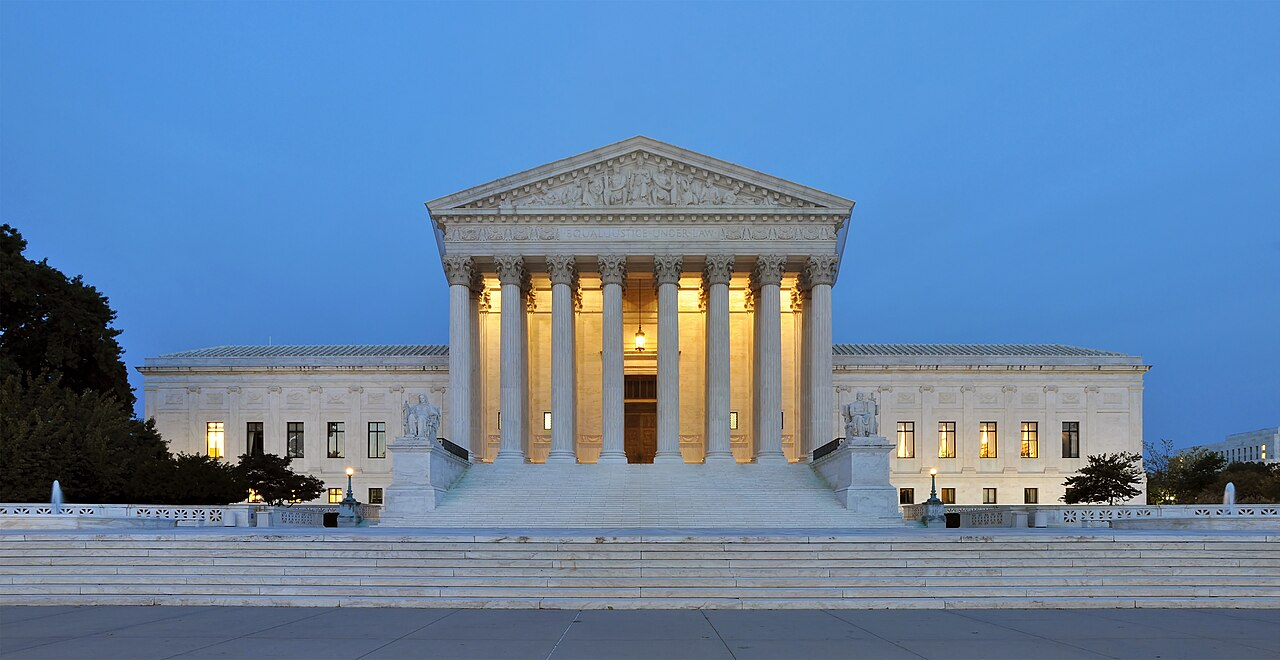
\includegraphics[width=\linewidth]{supreme_court.jpg}\\[-0.1em]
      {\tiny\color{muted} U.S. Supreme Court. Photo: Joe Ravi, CC BY-SA 3.0\par}
    \end{column}
  \end{columns}
\end{frame}

\begin{frame}{\emph{Barnette} (1943)}
  \vfill
  \begin{textquote}
    \Large ``If there is any fixed star in our constitutional constellation, it is that no official, high or petty, can prescribe what shall be orthodox in politics, nationalism, religion, or other matters of opinion or force citizens to confess by word or act their faith therein.''
  \end{textquote}
  \hfill --- Justice Robert H.\ Jackson, majority opinion
  \vfill
\end{frame}

\begin{thinkframe}
  {\color{oldred}\textbf{Think}}\\[0.8em]
  What part of American culture or law\\
  might lead the Supreme Court to this decision?
\end{thinkframe}

% =====================================================================
\section{Separation of Church and State}

\begin{frame}{The First Amendment (1791)}
  \vfill
  \begin{textquote}
    \Large ``Congress shall make no law respecting an \alert{establishment of religion}, or prohibiting the \alert{free exercise} thereof; or abridging the freedom of speech, or of the press \ldots''
  \end{textquote}
  \vfill
  \begin{itemize}
    \item \textbf{Establishment clause:} no official state religion
    \item \textbf{Free exercise clause:} everyone may practice (or not practice) any religion
  \end{itemize}
  \vfill
\end{frame}

\begin{frame}{Text Analysis}
  \begin{minipage}[c]{0.86\textwidth}
    {\small\color{muted} Thomas Jefferson, \emph{Letter to the Danbury Baptist Association}, 1802}
  \end{minipage}\hfill
  \begin{minipage}[c]{0.1\textwidth}
    \raggedleft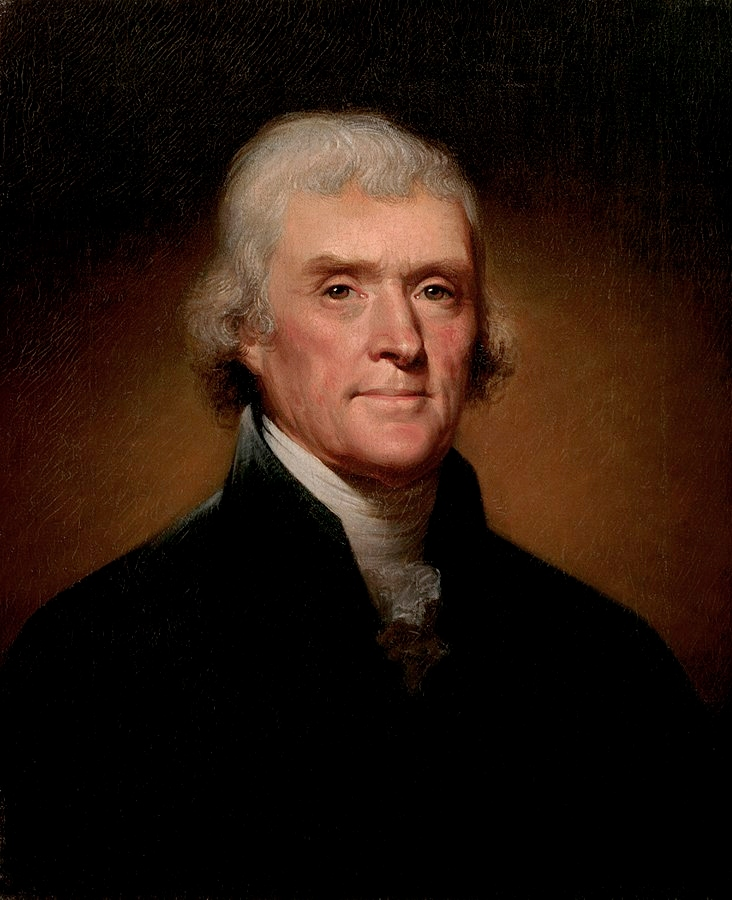
\includegraphics[height=1.25cm]{jefferson.jpg}
  \end{minipage}
  \vspace{0.2em}
  \begin{textquote}[fontupper=\itshape\footnotesize]
    ``Believing with you that religion is a matter which lies solely between Man \& his God, that he owes account to none other for his faith or his worship, that the legitimate powers of government reach actions only, \& not opinions, I contemplate with sovereign reverence that act of the whole American people which declared that their legislature should `make no law respecting an establishment of religion, or prohibiting the free exercise thereof,' thus building \textbf{a wall of separation between Church \& State}. Adhering to this expression of the supreme will of the nation in behalf of the rights of conscience, I shall see with sincere satisfaction the progress of those sentiments which tend to restore to man all his natural rights, convinced he has no natural right in opposition to his social duties.''
  \end{textquote}
\end{frame}

\begin{frame}{Church and State in Austria vs.\ the US: at school}
  \small
  \renewcommand{\arraystretch}{1.3}
  \begin{tabular}{@{}p{0.45\textwidth}p{0.49\textwidth}@{}}
    \toprule
    \textbf{\color{austria}In Austria} & \textbf{\color{oldblue}In the US} \\
    \midrule
    A cross must hang in every classroom where most students are Christian
      & Unconstitutional (\emph{Stone v.\ Graham}, 1980) --- though new Ten Commandments laws in Louisiana and Texas are being fought in court \\
    Religion class in public schools, taught by teachers approved by the church and paid by the state
      & Schools may teach \emph{about} religion, but not practice it; no school prayer (\emph{Engel v.\ Vitale}, 1962) \\
    The state pays the teachers at Catholic private schools
      & Very limited public money for religious schools \\
    \bottomrule
  \end{tabular}
\end{frame}

\begin{frame}{Church and State in Austria vs.\ the US: public life}
  \small
  \renewcommand{\arraystretch}{1.15}
  \begin{tabular}{@{}p{0.45\textwidth}p{0.49\textwidth}@{}}
    \toprule
    \textbf{\color{austria}In Austria} & \textbf{\color{oldblue}In the US} \\
    \midrule
    Church contribution (\emph{Kirchenbeitrag}) required by a state law; churches can sue members who don't pay
      & Churches are private and live on voluntary donations \\
    16 officially recognized religious communities; a 1933 treaty with the Vatican (\emph{Konkordat}) is still in force
      & The government does not recognize or rank religions \\
    Most public holidays are Catholic (Corpus Christi, Assumption, All Saints, \ldots)
      & Christmas is the only religious federal holiday \\
    Shops closed on Sundays
      & Most shops open; rare Sunday-closing laws are allowed only for non-religious reasons (``a day of rest'') \\
    \bottomrule
  \end{tabular}
\end{frame}

\begin{frame}{The American paradox}
  \begin{itemize}\setlength{\itemsep}{1em}
    \item The US separates church and state much more strictly than Austria \ldots
    \item \ldots\ yet Americans are \alert{far more religious} than Austrians
      \begin{itemize}
        \item ``In God We Trust'' is printed on every dollar bill
        \item Presidents end speeches with ``God bless America''
        \item ``under God'' is in the Pledge
      \end{itemize}
    \item \textbf{Discuss:} How does the separation of church and state change American culture? Could it even make religion \emph{stronger}?
  \end{itemize}
\end{frame}

% =====================================================================
\section{Drinking Culture}

\begin{frame}{Who drinks?}
  \begin{columns}[c]
    \begin{column}{0.48\textwidth}
      \begin{itemize}\setlength{\itemsep}{0.8em}
        \item Only \alert{54\%} of Americans drink alcohol --- tied for a record low (Gallup, 2026)
          \begin{itemize}
            \item 71\% in the 1970s; 62\% as recently as 2023
          \end{itemize}
        \item Austria: around \alert{90\%}
        \item Legal drinking age:
          \begin{itemize}
            \item US: \textbf{21}
            \item Austria: \textbf{16} (beer \& wine), \textbf{18} (spirits)
          \end{itemize}
      \end{itemize}
    \end{column}
    \begin{column}{0.5\textwidth}
      \centering
      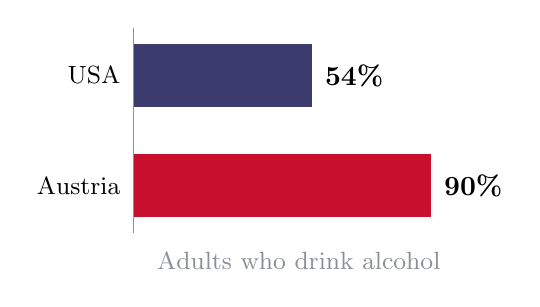
\begin{tikzpicture}[x=0.042cm]
        \foreach \y/\lab/\val/\col in {1.4/USA/54/oldblue, 0/Austria/90/austria} {
          \fill[\col] (0,\y) rectangle (\val,\y+0.8);
          \node[anchor=east, font=\small] at (-1,\y+0.4) {\lab};
          \node[anchor=west, font=\bfseries] at (\val+1,\y+0.4) {\val\%};
        }
        \draw[muted] (0,-0.2) -- (0,2.4);
        \node[font=\small, text=muted] at (50,-0.55) {Adults who drink alcohol};
      \end{tikzpicture}
    \end{column}
  \end{columns}
  \source{Sources: Gallup Consumption Habits poll (July 2026); Narconon Europe.}
\end{frame}

\begin{thinkframe}
  {\color{oldred}\textbf{Think}}\\[0.8em]
  Why might this be?
\end{thinkframe}

\begin{frame}{Explanation 1: Cannabis}
  \begin{columns}[c]
    \begin{column}{0.5\textwidth}
      \begin{itemize}\setlength{\itemsep}{0.8em}
        \item 24 U.S. states have legalized cannabis for recreational use
        \item \alert{17\%} of U.S. adults use marijuana (Gallup)
        \item Only \alert{6.3\%} of Austrian adults (EUDA)
        \item In Austria, cannabis is still illegal --- while Germany partly legalized it in 2024
      \end{itemize}
    \end{column}
    \begin{column}{0.48\textwidth}
      \centering
      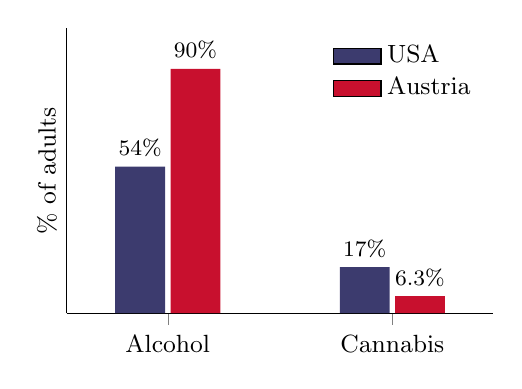
\begin{tikzpicture}
        \begin{axis}[
            ybar, width=7cm, height=5.2cm,
            ymin=0, ymax=105, bar width=18pt,
            symbolic x coords={Alcohol,Cannabis}, xtick=data,
            enlarge x limits=0.45,
            axis lines*=left, ytick=\empty,
            ylabel={\small \% of adults},
            nodes near coords={\pgfmathprintnumber\pgfplotspointmeta\%},
            every node near coord/.append style={font=\footnotesize},
            legend style={draw=none, fill=none, font=\small, at={(0.98,0.98)}, anchor=north east},
            legend cell align=left, area legend,
            ticklabel style={font=\small}]
          \addplot[fill=oldblue, draw=none] coordinates {(Alcohol,54) (Cannabis,17)};
          \addplot[fill=austria, draw=none] coordinates {(Alcohol,90) (Cannabis,6.3)};
          \legend{USA, Austria}
        \end{axis}
      \end{tikzpicture}
    \end{column}
  \end{columns}
  \source{Sources: Gallup; European Union Drugs Agency (EUDA). Survey definitions differ slightly between sources.}
\end{frame}

\begin{frame}{Explanation 2: Alcohol is seen as unhealthier}
  \relax{\small\color{muted} Text Analysis: Bernhard Maisch, ``Alcohol consumption --- none is better than a little,'' \emph{Herz}\par}
  \vspace{0.3em}
  \begin{textquote}[fontupper=\itshape\footnotesize]
    ``For several decades, epidemiological studies suggested that drinking alcohol in moderate quantities was beneficial. This was referred to as the `French paradox,' which described differences in mortality between France and Finland mainly, but also other countries, that were found in epidemiological studies. The difference in the levels of alcohol consumption was found to explain the differences in mortality in view of the otherwise similar risk factors. When alcoholic drinks per day were plotted against all-cause mortality this led to a J-shaped curve. This finding represented a window of benefit for moderate alcohol consumption. However, the recent publication by Zhao et al.\ in 2023 revisited the relationship between the quantity of alcohol consumed and mortality risk and led to a paradigm change, which has influenced not only the recommendations of Canada's Guidance on Alcohol and Health but also the recommendations and guidelines of major health organizations: \textbf{`No alcohol is better than a little.'}\,\ldots''
  \end{textquote}
\end{frame}

\begin{frame}{Explanation 2: Alcohol is seen as unhealthier}
  \relax{\small\color{muted} Text Analysis (continued)\par}
  \vspace{0.3em}
  \begin{textquote}[fontupper=\itshape\footnotesize]
    ``\ldots\ The J-shaped curve as an explanation of the French paradox became a linear relationship between the amount of alcohol consumption and the increasing mortality from tumors and cardiovascular diseases. The renewed review of several control groups in previous epidemiological studies revealed a recruitment error due to the inclusion of abstinent ex-drinkers. Taking this bias into account, the alcohol-friendly view of small amounts of alcohol being cardioprotective had to be revised. The combined misuse of alcohol and other risk factors for carcinogenesis and heart diseases still needs further attention. The misuse of both alcohol and cocaine led to the conclusion that when the two risky substances are consumed together, it is even more detrimental than the mere sum of the two.''
  \end{textquote}
\end{frame}

\begin{frame}{From a J-curve to a straight line}
  \centering
  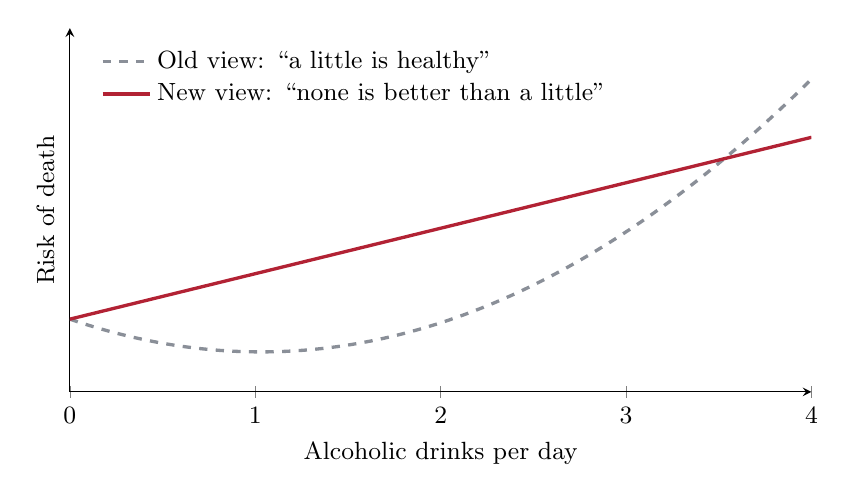
\begin{tikzpicture}
    \begin{axis}[
        width=11cm, height=6.2cm,
        xmin=0, xmax=4, ymin=0.6, ymax=2.6,
        axis lines=left, xtick={0,1,2,3,4}, ytick=\empty,
        xlabel={Alcoholic drinks per day}, ylabel={Risk of death},
        legend style={draw=none, fill=none, at={(0.03,0.97)}, anchor=north west, font=\small},
        legend cell align=left, ticklabel style={font=\small}, label style={font=\small}]
      \addplot[domain=0:4, samples=80, very thick, muted, dashed] {1 - 0.35*x + 0.17*x^2};
      \addplot[domain=0:4, samples=2, very thick, oldred] {1 + 0.25*x};
      \legend{Old view: ``a little is healthy'', New view: ``none is better than a little''}
    \end{axis}
  \end{tikzpicture}

  {\tiny\color{muted} Schematic illustration, not real data.}
\end{frame}

\begin{frame}{Official advice: USA vs.\ Austria}
  \begin{columns}[T]
    \begin{column}{0.48\textwidth}
      \textbf{\color{oldblue}USA}
      \begin{itemize}\setlength{\itemsep}{0.6em}
        \item \emph{``People who do not drink should not start drinking for any reason.''}\\
          {\footnotesize\color{muted} --- Dietary Guidelines for Americans, 2020--2025}
        \item 2025: the U.S.\ Surgeon General calls for cancer warning labels on alcohol
        \item 51\% of Americans now say 1--2 drinks a day are \emph{bad} for your health (Gallup, 2026)
      \end{itemize}
    \end{column}
    \begin{column}{0.48\textwidth}
      \textbf{\color{austria}Austria}
      \begin{itemize}\setlength{\itemsep}{0.6em}
        \item ``Low-risk'' limit: \textbf{24\,g of alcohol per day} for men, 16\,g for women
        \item 24\,g $\approx$ \textbf{0.6\,L of beer} --- every day
      \end{itemize}
    \end{column}
  \end{columns}
\end{frame}

% =====================================================================
\section{Living to Work or Working to Live?}

\begin{frame}{Time at work}
  \centering
  \renewcommand{\arraystretch}{1.5}
  \begin{tabular}{@{}lcc@{}}
    \toprule
    & \textbf{\color{oldblue}USA} & \textbf{\color{austria}Austria} \\
    \midrule
    Paid time off (vacation) & 10--15 days (average) & \textbf{25 days} (legal minimum) \\
    Legal minimum vacation & \alert{none} & 5 weeks \\
    Hours worked per year & 1,765 & 1,611 \\
    \bottomrule
  \end{tabular}

  \vspace{2em}
  \begin{itemize}
    \item \textbf{Guess:} Which countries work the \emph{fewest} and the \emph{most} hours?
      \only<2>{\\[0.3em]\alert{Fewest: Germany \quad Most: Sudan}}
  \end{itemize}
\end{frame}

\begin{frame}{Money}
  \centering
  \renewcommand{\arraystretch}{1.5}
  \begin{tabular}{@{}lcc@{}}
    \toprule
    & \textbf{\color{oldblue}USA} & \textbf{\color{austria}Austria} \\
    \midrule
    Average yearly wage & \$86,977 & \$78,301 \\
    GDP per person & \$95,212 & \$61,080 \\
    \bottomrule
  \end{tabular}

  \vspace{2.5em}
  \pause
  \begin{columns}[c]
    \begin{column}{0.4\textwidth}
      \centering
      {\fontsize{40}{44}\selectfont\bfseries\color{oldred} 989}\\[0.2em]
      {\small of the world's 3,248 billionaires are American}
    \end{column}
    \begin{column}{0.4\textwidth}
      \centering
      {\fontsize{40}{44}\selectfont\bfseries\color{navy} 30\%}\\[0.2em]
      {\small of billionaires --- but only about 4\% of the world's population}
    \end{column}
  \end{columns}
\end{frame}

\begin{thinkframe}
  {\color{oldred}\textbf{Think}}\\[0.8em]
  What does this tell us about\\
  American and Austrian working cultures?
\end{thinkframe}

% =====================================================================
\section{Activity: Spectrum Game}

\begin{frame}{Spectrum Game}
  \begin{itemize}\setlength{\itemsep}{1em}
    \item You will see a series of statements
    \item Stand somewhere in the room to show how much you \alert{agree or disagree}
    \item Be ready to explain your position!
  \end{itemize}
  \vfill
  \begin{center}\spectrum\end{center}
  \vspace{0.8cm}
\end{frame}

\statement{1}{A culture of social drinking is a good thing.}
\statement{2}{The government should not express\\any religious views.}
\statement{3}{Shops being closed on Sundays is a good thing,\\regardless of one's religion.}
\statement{4}{It is important to be loyal to one's country.}
\statement{5}{Work should be the main source\\of fulfillment in one's life.}

\begin{thinkframe}
  Thank you!\\[0.4em]
  {\large Questions?}
\end{thinkframe}

\end{document}
